\documentclass[10pt]{report}

\usepackage{ mathrsfs }

\usepackage[utf8]{inputenc}
\usepackage[LGR,T1]{fontenc} % this is to be able to output greek 

%\renewcommand*\rmdefault{stix} % change the font
% \usepackage{times} % use times font for report

\usepackage{setspace} % pour agrandir l'interligne
% \doublespacing pour double espace sinon \onehalfspacing pour 1.5

\usepackage{geometry} % Required to change the page size to A4
\geometry{a4paper} % Set the page size to be A4 as opposed to the default US Letter

\usepackage{graphicx} % Required for including pictures

\usepackage{float} % Allows putting an [H] in \begin{figure} to specify the exact location of the figure
\usepackage{wrapfig} % Allows in-line images

\usepackage{parskip}

\usepackage{amsmath} % Package to use the \text in equation environement
\usepackage{amssymb} %Package for fancy math symbols

\usepackage[style=authoryear]{biblatex} % Using biblatex package for bibiography in order to comply with INSA requirements
\setlength\bibitemsep{1.25\itemsep} % adding space between bib entriesS

\makeatletter

\newrobustcmd*{\parentexttrack}[1]{%
  \begingroup
  \blx@blxinit
  \blx@setsfcodes
  \blx@bibopenparen#1\blx@bibcloseparen
  \endgroup}

\AtEveryCite{%
  \let\parentext=\parentexttrack%
  \let\bibopenparen=\bibopenbracket%
  \let\bibcloseparen=\bibclosebracket}

\makeatother

\addbibresource{biblio.bib}

\newcommand{\textgreek}[1]{\begingroup\fontencoding{LGR}\selectfont#1\endgroup} % type greek words

% redefine the chapter style
\usepackage{titlesec, blindtext, color}
\definecolor{gray75}{gray}{0.75}
\newcommand{\hsp}{\hspace{20pt}}
\renewcommand{\thechapter}{\Roman{chapter}}
\titleformat{\chapter}[hang]{\Huge\bfseries}{\thechapter\hsp\textcolor{gray75}{|}\hsp}{0pt}{\Huge\bfseries}

\usepackage{graphicx} % Required for including pictures
\graphicspath{{art/}} % Specifies the directory where pictures are stored

\usepackage{framed} % to frame the project title

\usepackage{datetime} % print dates

\usepackage{lipsum} % Used for inserting dummy 'Lorem ipsum' text into the template

\usepackage{geometry}% http://ctan.org/pkg/geometry

\usepackage{fancyhdr} % for header and footer custom

\setcounter{secnumdepth}{3}  % to have subsubsections numbered
\renewcommand\thesubsection{\arabic{subsection}}
\renewcommand\thesubsubsection{\thesubsection.\alph{subsubsection}}


% ---------- Aliales, macros
\newcommand{\ochain}{$\otimes \text{-chain}$}
%---------------------------

\begin{document}

\setlength{\parindent}{1em}
\def\labelitemi{--} % defining dash instead of bullets

% -------------------------------- %
%            TITLE PAGE            %
% -------------------------------- %
\newgeometry{vmargin=1in}
\begin{titlepage}

\begin{center}


\includegraphics[width=2.5cm]{INSA-logo.jpg} \hspace{3cm}

\includegraphics[width=1.5cm]{NICTA-logo.jpg}\hspace{4cm}

\includegraphics[width=1.5cm]{IAE-logo.jpg} 

\vspace{3cm}
\textsc{\LARGE \textit{\textbf{\uppercase{End of studies project report}}}}
\vspace{1.5cm}

\begin{framed}
\LARGE \uppercase{Extension of a Business Process Compliance tool\\Revision of the Product's Strategy}
\end{framed}

\vspace{1cm}
\large En vue de l'obtention des diplomes \\
Ingénieur Informatique et Réseaux de l'INSA de Toulouse\\
Master Management de l'Innovation de l'IAE de Toulouse

\end{center}
\vspace{1.5cm}
\begin{flushright}
\textbf{\large  NICTA Queensland Research Laboratory\\ \hspace{.5cm}- Brisbane, QLD, Australia}
\end{flushright}

\vspace{1.3cm}
\begin{center}
\begin{minipage}{.3\textwidth}
\begin{center}
\textbf{INSA Tutor}\\
Nawal Guermouche\\
Researcher at the LAAS\\
nguermouche@laas.fr
\end{center}
\end{minipage}
\begin{minipage}{.3\textwidth}
\begin{center}
\textbf{NICTA Tutor}\\
Guido Governatori\\
Principal Researcher at the NICTA\\
governatori@nicta.com
\end{center}
\end{minipage}
\begin{minipage}{.3\textwidth}
\begin{center}
\textbf{IAE Tutor}\\
Margaret K. Kyle\\
Professor, UT1\\
margaret.kyle@iae-toulouse.fr
\end{center}
\end{minipage}
\end{center}

\vfill
\begin{minipage}{0.55\textwidth}
\begin{flushleft}
\textbf{\large Marc Allaire\\[.5cm] 
\small INSA - Spécialité Informatique et Réseaux,\\\hspace{.5cm}Majeure Systèmes Distribués Communicants\\
IAE - Master Management Stratégique,\\\hspace{.5cm}Spécialité Management de l'innovation}
\end{flushleft}
\end{minipage}
\begin{minipage}{0.4\textwidth}
\begin{flushright}
\newdate{date}{30}{08}{2014}
\textbf{\displaydate{date}}
\end{flushright}
\end{minipage}


\end{titlepage}




\newpage
\pagenumbering{gobble} % no page numbering until otherwise set by \pagenumbering{arabic}
% -------------------------------- %
%              REPORT              %
% -------------------------------- %
\restoregeometry
\renewcommand{\thesection}{\Roman{section}} 

%executive summary
\renewcommand{\abstractname}{Executive Summary}
\begin{abstract}
This report presents the work done around the Regorous software at NICTA during my final year internship. It is divided in two main parts. First a technical one that presents the new features that were added to the code-base. After a short but thorough introduction to the theoretical work underlying you will find an in-depth presentation of the new components that were implemented. My main contributions are : 
\begin{itemize}
\item Impementation of Cooccurrent obligation to extend the \enquote{vocabulary} available to translate regulation into defeasible rules. This necessitated a rewrite of the core library to introduce this new type and modify the compliance checking algorithm to take into account the special behaviour of this obligation.
\item Modifications of the implementation of the compliance checking algorithm to check compliance of compensation chains in the same task they were triggered in instead of waiting for the next task. 
\item Porting of the eclipse plug-in project to the current version of eclipse and third party libraries. This was an intensive work that taught me a lot about issues related to production environement. This is not something I was used to as a young graduate but the INSA generalist formation helped me go through.
\end{itemize}

Most of the code in this report is Java code or pseudo algorithmic code. I will not go into too much details about the exact implementation but rather focus on the methodology and the algorithms I used during the project.

~\\Second part is more strategy oriented, it is built around reviewing Regorous marketing strategy. Indeed, NICTA is not only working on technological matters but on how they can impact the \enquote{real world} and make it to production use in firms. There has been past attempts to sell the software to companies but all failed. I present an historical review of the work already done and try to build a product strategy based on past feedbacks and marketing studies.

I also investigate what are the side effects of Regorous and aim to link these with existing work taking its roots from both research and the corporate world. I present how Regorus is a great tool of knowledge management within the firm and back my argument with research papers.

The report finds that the lack of a proper marketing study for Regorus is leading to a lot of approximations and guesses when it comes to targeted market or individuals within the firm. There is an urgent need to pinpoint who are the decision makers in corporations when it comes to buying software and what are their motivation, who they listen to, what is important to them. In short, we must know who are our clients. I suggest a that a focus group should be done once the targeted audience is well defined and propose a collection of subjects that could be worked on.

\end{abstract}



\newpage

% special thanks
%executive summary
\begin{center}
\begin{minipage}{.8\textwidth}
\textbf{\large Acknowledgement}\\\\
I would like to take this opportunity to thank all the people who have contributed in some way to this reports particulary Mr Guido Governatori who initiated the project, for his attention, and for all the time he awarded to me, his advice was really useful and appreciated.\\

I also thank all the member of NICTA QRL who were always ready to help me. It was an amazing experience both humanely and professionally \\

Then, I would like to thank all the members of the Business Process Compliance group for their patience and the time they spent to explain their work to me.\\

\end{minipage}
\end{center}

\newpage
\setcounter{tocdepth}{3} % to have subsubsections in TOC
\tableofcontents
\newpage
\pagenumbering{arabic}
\setcounter{page}{1}
% \pagestyle{headings}
\pagestyle{fancy}
\renewcommand{\sectionmark}[1]{\markright{\thesection.\ #1}}
\fancyhead{}
\fancyhead[R]{\slshape \rightmark}
\fancyfoot{}
\fancyfoot[C]{\thepage}
\renewcommand{\headrulewidth}{0.4pt}
\renewcommand{\footrulewidth}{0 pt}

\chapter{Presenting the context of the Project}
\section{A brief presentation of NICTA}
NICTA is Australia's Information and Communication Technologies centre of excellence.\footnotemark It was created in 2002 within the framework of the Backing Australia's Ability initiative a government plan to foster innovation in Australia. NICTA won the selection process to become Australia's ICT centre of excellence. It is supported and funded by the Australian federal government as well as states governments where laboratories are running (New South Wales, Victoria, Queensland, Australian Capital Territory). Major universities in each of the previously cited states also participate in the funding.\\

\footnotetext{Centre of Excellence are a common term used by Australian government to qualify prestigious centre of expertise where researchers collaborate to maintain Australia's international standing in research areas of national priority \autocite{ARCCentreExcellence}}

NICTA has 5 laboratories around Australia and employs over 700 people representing the largest research organisation dedicated to ICT in Australia. Since its foundation it has developed many collaboration with the industry especially via joint projects and company creation. NICTA not only focuses on research excellence but is actively looking for business opportunities to capture the value created by its research group. Hence an organisation divided in two main centres \autocite{PresentationBooklet}.

\begin{description}
\item[Research Groups] are aiming to become leaders in their own domain of expertise with a long-term vision for ICT-innovation producing cutting edge results. Each operating in a different areas, they cover a large part of information and communication technologies. They are (in no particular order) :
\begin{itemize}
\item \textbf{Software Systems} is aiming to provide secure, reliable and safe systems that are proven to achieve \enquote{real world} enterprise performance and objectives. 
\item \textbf{Computer Vision} mainly work at a fundamental level in order to provide tools to better analyse the world through 2D videos. Their key areas of research are using the existing mathematics of multiple view geometry with new techniques such as machine learning and optimization.
\item \textbf{Control and Signal Processing} produces theoretical and algorithmic work leading to innovative methods and systems. The focus is set on two main domain of application decentralized control and estimation for large distributed systems as well as the convergence between computing science and biology.
\item \textbf{Optimization} is working on a new generation of optimization systems that will be operating in dynamic and noisy environment involving huge amounts of data.
\item \textbf{Machine Learning} develops new algorithms and technologies to make sense of the skyrocketing amount of data gathered in all areas of human endeavour. 
\item \textbf{Networks} is improving the user experience in current and next generation networked environment by developing new theories, models and methods.
\end{itemize}

\item[Business Teams] are focused on exploiting the results of research through active market exploration and strategic surveillance. They provide business support for researchers and therefore cover economic sectors related to the above research groups. They are (in no particular order) :
\begin{itemize}
\item \textbf{Broadband and the Digital Economy} promotes new digital technologies and services in all the Australian market : government, SME, enterprises and end-users.
\item \textbf{Health} develops and fosters the penetration of information technologies into the biological world leading to a better understanding of biological systems and diseases.
\item \textbf{Infrastructure, Transports and Logistics} provide innovative ICT solutions to radically improve transportation systems and infrastructure networks.
\item \textbf{Security and Environment} increases the security of critical and sensitive Australian infrastructure and reduces our impact on the environment.
\end{itemize}
\end{description}

\section{The Business Process Compliance Group}

The Business Process Compliance group in which I am working is part of the Software Systems group, one of the six research groups. The interest in business process compliance starts from a simple observation. ICT systems are costly and hard to develop because of the constantly evolving framework of norms and requirement within which they operate leading to less agility and slower development cycles especially in domains with strict legal obligations. Business process compliance is becomming an increasing area of concern in both public and private sectors because of the complexity of regulations and the lack of automated tools. The compliance market is worth tenth of billions of dollars in Australia.\autocite{BPCWebsite}

From this observation, the BPC group started by selecting a framework to represent both business processes and the laws they must comply to. These research lead to numerous articles aiming to build a model of rules and business processes that would give the end user the most flexibility and the possibility to accurately translate existing body of law. This theoretical work led to more concrete projects. As of today the group in undergoing three main projects~: Regorous, SPINdle and the Rule Editor. These provide a powerful platform for compliance officers in companies.


\newpage
\chapter{Technical work on Regorus}
\section{Introducing the project's theoretical framework}
\subsection{A short introduction to defeasible logic}

Defeasible reasoning as presented in \autocite{koons_defeasible_2005} is a non-demonstrative type of reasoning where one cannot reach a full, undoubted conclusion and where a conclusion can be defeated if further evidence of the contrary is demonstrated. Both computer scientists and philosophers has shown an interest in this field. The philosophical interest can be traced back to ancient Greece and Aristotle. Although the scientific reasoning is built on deductive logic, for everyday life we rely on a defeasible reasoning. We try to make general statements out of personal experience, for example we could say that all birds fly. This proposition would be true until we experience a bird that cannot fly such as a penguin. This would defeat the first rule.

Computer scientist interest in defeasible logic has grown during the last 40 years especially in the field of artificial intelligence. An intelligent program needs a formal representation of the world, a formal language to represent knowledge, causality and ability in order to achieve its given goal. This requirement was first introduced in \autocite{mccarthy1968some}.

Defeasible Logic was first introduced by Donal Nute in \autocite{nute1994defeasible} as a proposition to represent defeasible reasoning in a logical way. As stated in \autocite{ecai2000} defeasible logic is a flexible non-monotonic formalism able to represent a large set of non-monotonic reasoning. Also several powerful implementations have been proposed with good complexity properties allowing a correct computational time. This has been made possible by the design of defeasible logic that makes implementation easy yet efficient.

Let's introduce the basics of Defeasible Logic as in \autocite{RepresentationResultsDefeasibleLogic}. A defeasible theory gives us five different ways of representing knowledge \textit{facts}, \textit{strict rules}, \textit{defeasible rules}, \textit{defeaters} and a \textit{superiority relation}. 

\begin{description}
\item[Facts] are indisputable statements for example Tux is a penguin which could be written formaly as $penguin(Tux)$
\item[Strict rules] are rules as in deductive logic. It's the kind of rule we find in scientific reasoning. The conclusion is irrefutable if the premises also are. These are formally represented as : 
$$penguin(X) \rightarrow bird(X)$$
\item[Defeasible rules] are the ones that can be defeated by evidence of the contrary. To draw a parallel with everyday reasoning one could generalize from experience that "Birds fly" a statement that would be true until the opposite is deducted. These rules are formally represented as :
$$bird(X) \Rightarrow flies(X)$$
\item[defeaters] are weaker rules that cannot be used to draw any conclusion but can prevent one. They are used to defeat other rules (hence the name) because they produce evidence of the contrary. 
$$heavy(X) \leadsto \neg flies(X)$$
From this defeater we cannot conclude that because someone or something is heavy it cannot fly, it is only here to prevent the conclusion of $flies(X)$.
\item[Superiority relation] is used to create an order in a rule set. It is important to note that this relation does not have the properties of a proper superiority relation. When we have two different rules which derive something and its negation we cannot draw a conclusion since defeasible logic is skeptical. The superiority relation allows us to come to a conclusion. For example :

\[
\begin{aligned}
& r :&      bird(X) &\Rightarrow flies(X)\\
& r':&brokenWing(X) &\Rightarrow \neg flies(X)\\
& & r'>r
\end{aligned}
\]

In this case we cannot reach a conclusion since $r$ and $r'$ reach opposite concusions. By introducing the superiority relation we say that $r'$ is stricly stronger than $r$ and therefore we can conclude that the bird cannot fly. Please note that there is no cyclical 
\end{description}

Now that we are more familiar with the concepts of defeasible logic we can show how we can reach a defeasible conclusion using proof theory. It exists four proof types for a conclusion D.
\begin{description}
\item[$\pm\Delta$q] means that $q$ or $\neg q$ or is definitely provable in D
\item[$\pm\partial$q] means that $q$ or $\neg q$ or is defeasibly provable in D
\end{description}

We won't get into details about how to definitely prove a literal since the focus of this report is more on defeasible proof. All you need to know is that if $q$ is definitely provable then it is also defeasibly provable.

In \autocite{RepresentationResultsDefeasibleLogic} provability is defined using the concept of \emph{derivation} in a conclusion D which is a set of facts rules and superiority relations ($D=(F,R,>)$). A derivation P can be seen as several steps in a demonstration. At the step $P(i)$ of the proof we have a given set $(F,R,>)$ from this we can prove $P(i+1)$ either definitely or defeasibly.

In order to reach a definitive conclusion $\pm\Delta q$ we need to have a rule that deduce $(\neg)q$ or have $(\neg)q$ as a fact. 

The following definitions exposes how to defeasibly conclude a literal $q$ at $P(i+1)$.
\newtheorem{mydef}{Definition}
\begin{mydef} \label{def-defeasible-proof}
If $P(i+1)$ = $+\partial q$ then either
\begin{enumerate}
\item $+\Delta q$ $\in$ $P(1..i)$ or
\item \begin{enumerate}
      \item $\exists r$ $\in$ $R_{sd}[q]$, $\forall a$ $\in$ $A(r)$ : $+\partial a$ $\in$ $P(1..i)$
      \item $-\Delta q$ $\in$ $P(1..i)$
      \item $\forall s$ $\in$ $R[\neg q]$ either
          \begin{enumerate}
          \item $\exists a$ $\in$ $A(s)$ : $-\partial a$ $\in$ $P(1..i)$ or
          \item $\exists t$ $\in$ $R_{sd}[q]$ such that \\ $\forall a$ $\in$ $A(t)$ : $+\partial a$ $\in$ $P(1..i)$ and $t>s$
          \end{enumerate}
      \end{enumerate}
\end{enumerate}


\end{mydef}

In less mathematical terms this definition means that in order to defeasibly prove $q$ we can follow two paths. Either prove that $q$ is definitely provable or work the defeasible part. Three conditions apply :
\begin{enumerate}
\item there is a rule r that concludes $q$ for every literal $a$ such as $a$ has been defeasably proven in a previous step $P(1..i)$.
\item $\neg q$ has not been definitively proven in a previous step $P(1..i)$
\item for every rule $s$ that conclude $\neg q$ for a literal $a$ either
  \begin{enumerate}
  \item $\neg a$ has been defeasibly proven in a previous step $P(1..i)$ or
  \item there is a rule $t$ that concludes $q$ such as $t>s$
  \end{enumerate}
\end{enumerate}


\subsection{Using defeasible deontic logic to represent legal norms and regulations}

Regulations and legal norms are an important concern for government and businesses. They are complex and hard to reason about especially when multiple regulations written separately are applied to a given situation. In a world where compliance to regulation is becoming both harder and more important because of their growing number and sanctions applied for non compliance, a normative logical framework is needed to be able to reason about regulations.

Deontic logic (from ancient greek \textgreek{deontos} meaning duty, what must be done) is a branch of symbolic logic concerned with the logic of obligations and permissions \autocite{mcnamara_deontic_2010}. Therefore it is exactly the kind of logical framework we want to be able to express regulations. Unfortunately standard deontic logic is unable to represent simple notions of normative reasoning such as prima-facie obligations or contrary-to-duty obligation. This lack of expressibility has driven away the very people that would have used deontic logic the most\autocite{nute1997defeasible}.

Let's take a closer look at prima-facie obligation for example and see how we can express these in the light of defeasible logic. Prima-facie means \enquote{at first sight} hence a prima-facie obligation is an obligation that stands at first sight, one that can be defeated if new facts can prove otherwise. We can see that this type of obligation can easily be expressed using defeasible logic, it is defeasible. Furthermore regulations contain feature exceptions that are easily represented using defeasible logic.

There are many benefits to use a logical framework to represent regulations, some of those are presented in \autocite{ModellingAndAnalysisOfRegulations}. They are subdivided into two main area of application :
\begin{itemize}
\item \textbf{the understanding and application of regulations} for users not familiar with legal writing and don't want to study a regulation yet being under the obligation to comply.
   \begin{description}
   \item \textit{Decision support} : If I make this decision, is it compliant ? You can run your process against a set of regulations and see if it complies. This is one of the situations where Regorous is actually effective. A formal framework for expressing processes is needed too in this case.
   \item \textit{Explanation} : We can return to the user the complete reasoning chain that lead to the given answer. It is therefore easier for the user to understand what cause this answer for their request.
   \end{description}
\item \textbf{the creation of regulation} for assisting legal professional in their work.
   \begin{description}
   \item \textit{Anomaly detection} Having a formal logical framework backing the drafting of regulation allows us to easily detect anomalies such as inconsistencies or loops.
   \item \textit{Hypothetical reasoning} It is possible, like for decision support, to inspect the effects of a regulation on the entire system.
   \item \textit{Debugging} When a regulation is not yielding the expected answer to a given query it is possible to debug it.
   \end{description}    
\end{itemize}

\subsubsection{Different types of obligations}
Now that we explained the need for a logical framework for legal reasoning and how good deontic defeasible logic is we can introduce the different types of obligations. Indeed to accurately represent the complexity of norms and regulations it is necessary to have a range of different types of obligations to be able to translate legal text into an equivalent logical representation as explained in \autocite{ConceptuallyRichModelofBPC}. There is three main types of obligations :
\begin{itemize}
\item \textbf{Achievement Obligation} : There is an obligation to meet once before the deadline. For example \textit{You must change your tires before they are worn out}
\item \textbf{Maintenance Obligation} : There is an obligation to meet at all instant before the deadline. For example \textit{You must provide for your children until they are 18}
\item \textbf{Punctual Obligation} : There is an obligation to meet at one instant. They must be fulfilled at the same moment they were triggered.
\end{itemize}

Achievement obligations can be further detailled to be able to express what happens if a violation of the obligation occurs. Does the obligation persists ? (\textit{You must pay the fine within 90 days otherwise you must pay a 15\% tax.} In this case it is obvious that the obligation to pay the fine is persistant after the deadline, after it was violated.) We therefore introduce a new concept that can apply to an achievement obligation : \textbf{Persistant or non Persistant}

We still lack vocabulary to express another subtlety of achievement obligations. Let's consider the following obligation \textit{When shopping for an item a consumer must pay for it after receiving the invoice and no later than 30 days after receiving it.} Now if the customer by mistake or for any other reason transfers the due amount before receiving the invoice. Then it is obvious that the obligation has been fulfilled even though the action was take outside of the time frame allocated to it. We will call this type of obligation \textbf{Preemptive and non-Preemptive}. 

Also, please note that these concepts cannot apply to maintenance or punctual obligations.

The following table summarizes the aforementioned concepts and the notation attached to it.

\renewcommand{\arraystretch}{1.5}
\begin{center}
\begin{tabular}{c|c|c}
Operator & Inline Notation & Read as \\
\hline
$O^{a, \pi}_{pr}$     & [OAPP]  & Achievement Persistent Preemptive            \\
$O^{a, \pi}_{n-pr}$   & [OAPNP] & Achievement Persistent non-Preemptive        \\
$O^{a, \tau}_{pr}$    & [OANPP]  & Achievement non-Persistent Preemptive        \\
$O^{a, \tau}_{n-pr}$  & [OANPNP]  & Achievement non-Persistent non-Preemptive    \\
$O^{m}$               & [OM]  & Maintenance                                  \\
$O^{p}$               & [OP]  & Punctual                                     \\
\end{tabular}
\end{center}

\subsubsection{Expressing chain of obligation with the $\otimes$ operator}

Now that we described the broad range of obligation giving us the necessary vocabulary to translate regulations into our logical framework. Still we are missing one critical point of regulations : reparation chains. If an obligation is violated, you are not complying with the regulation unless there is a reparation chain that kicks in and leaves you in an unoptimal situation compliance wise but still compliant.

 For example let's consider the following rules : 
 \[
 \begin{aligned}
   & r : &\text{invoice} & \Rightarrow O^{a, \pi}_{pr}\text{pay}\\
   & r': &\neg \text{pay} & \Rightarrow O^{p}\text{pay fine}
 \end{aligned}
 \]
 Well it can be reduced to be expresses as a $\otimes$-expression such as these two obligation cannot be seen any more as independent. 
  \[
 \begin{aligned}
   & r : &\text{invoice} & \Rightarrow O^{a, \pi}_{pr}\text{pay} \otimes O^{p}\text{pay fine}\\
 \end{aligned}
 \]

We can now create chains of obligations started by a given set of literal and giving the actor a chance to stay compliant even if an obligation was violated. \autocite{NormComplianceinBPModeling}

\subsection{BPMN2.0 and the representation of business processes}
Business process are 



\subsection{Tools already developed : Regorus and SPINdle}
What are they and what are they doing ?\\
Areas of improvement ?


\newpage
\section{Adding features to Regorus}
\subsection{Implementing Cooccurrent Obligations}
As introduced earlier there is different types of obligation in defeasible logic. This wide range allows us to model precisely and accurately a large number of business processes and rules. However some shortcomings have been spotted leading to imprecise modelling.

Let's first introduce an example to underline the lack of appropriate obligation. Taken from the Australian \textbf{INSERT THE PROPER ACT HERE} act when needing personal information from someone it must be given by the person himself. We could model this rule with a punctual obligation like this :
\begin{equation}
r1 : \text{Need Personal Information} \Rightarrow \text{[Op] Get it in person}
\end{equation}
In the current implementation of the compliance checking algorithm if the effect of the task triggers the rule $r1$ then the obligation is carried on to the next task where it will be checked in the \textit{Current} obligation set. In our example that does not really make sense since once we get the information we should check \textbf{in the same task} is the information was taken personally or not.

To be able to precisely describe this kind of behaviour we need to introduce a new type of obligation, Cooccurrent Obligation. This represent an extension of punctual obligation which must be fulfilled in the same task where it was triggered. The addition of this new obligation forces us to modify the implementation of the software in the core packages to check compliance as well as in the editor part to let the user add this kind of obligation to their implementation of rules.

First let's see how this new type changes the core compliance checking algorithm :

For now the compliance checking algorithm works in five main steps for each task of the business process :
\begin{enumerate}
\item Get the obligations generated from the previous task
\item Get the effects of the current task
\item Generate new effects
\item Check compliance with the given obligations and effects
\item Generate the new obligations for the next task
\end{enumerate}

We need to make a few changes to take into account the new type of obligation. First, in the generated obligations look for Cooccurrent obligations then check these obligations on the literals just generated and see if there is a violation. If this is the case then the chain of reparation is marked as activated and checked for compliance in the task.

As we said before cooccurrent obligations are close relatives of punctual obligations this allows us to leave the compliance checking algorithm and related routines unchanged and just call it again with the freshly generated cooccurrent obligation as punctual obligations and the new effects. To sum up we add three new steps to the pseudo algorithm introduced previously :
\begin{enumerate}
\item Get cooccurrent obligation from the set of new obligations
\item Call the compliance checking algorithm to check compliance with the new effects and the cooccurrent obligations
\item Generate new obligations for the next task and forward
\end{enumerate}

Now we need to take into account violation and compensation. If a cooccurrent obligation is violated and if it is part of a compensation chain we will check the rest of the chain in the very same task it was activated.



\subsection{XOR splits and the condition associated to them}
In order to be able to implement conditional splits in business processes it is necessary to have XOR splits and corresponding XOR join. Unfortunately with this mandatory tool for business process modelling comes some issues, especially with punctual obligations, that we will try to tackle.

First let see how XOR nodes behave in business process modelling with a little example from a demonstration video of Regorus \autocite{regorusVid}.

\begin{figure}[!h] %on ouvre l'environnement figure
\begin{center}
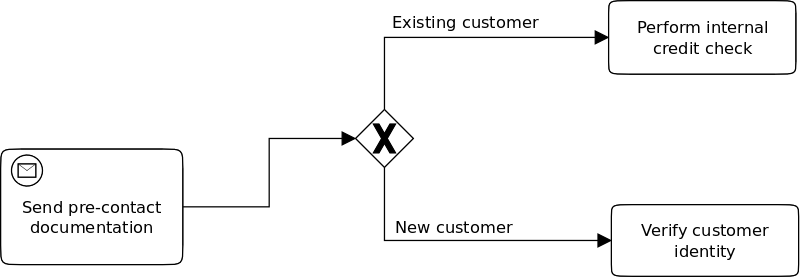
\includegraphics[height=3.4cm]{XOR.png} %ou image.png, .jpeg etc.
\caption{A simple example of XOR split} %la légende
\end{center}
\label{image_soleil} %l'étiquette pour faire référence à cette image
\end{figure} %on ferme l'environnement figure 

This sample shows an important feature of the XOR nodes : annotations on the edges. When checking compliance all the possible executions of a given business process are computed which mean in one case we will have \textit{Existing Customer} as an effect and in another thread we will have \textit{New Customer} as effect. The issue is in the way we take these effects into account to check compliance in the following tasks.

For now Regorus puts \enquote{dummy nodes} between the XOR split and the first task as shown in the following illustration.
\begin{figure}[!h] %on ouvre l'environnement figure
\begin{center}
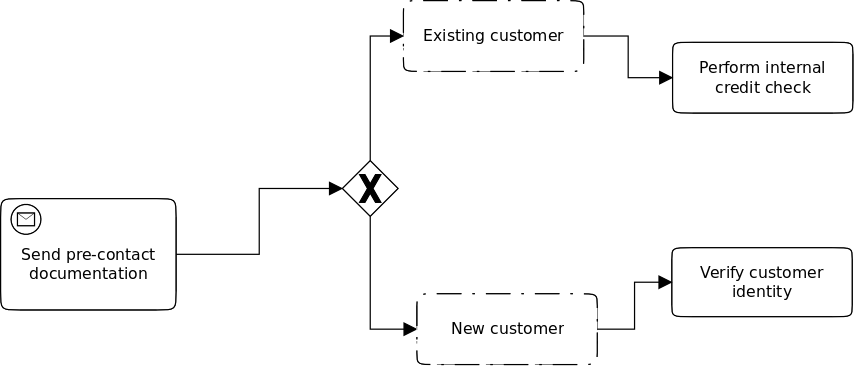
\includegraphics[height=4cm]{XOR2.png} %ou image.png, .jpeg etc.
\caption{Illustration of the \enquote{dummy nodes} added by regorus} %la légende
\end{center}
\label{image_soleil} %l'étiquette pour faire référence à cette image
\end{figure} %on ferme l'environnement figure

But a better behaviour would be to take these directly into account without the need for dummy nodes. Indeed punctual and cooccurrent obligations cannot be handled properly in this case. If the node before the XOR split yields an punctual obligation like this one $\text{p} \rightarrow \text{[Op]q}$ then with the actual implementation the obligation will be checked in the dummy nodes when it should be checked for compliance in the first \enquote{real} node following the XOR split.

Again for cooccurrent obligations if the effect associated with the edge of the XOR split yields a cooccurrent obligation like $\text{p} \rightarrow \text{[Oc]q}$ then it will be checked on the dummy node when it should, once again, be checked for compliance in the first \enquote{real} node following the XOR split.

We chose to follow these steps to implement this desired behaviour :
\begin{enumerate}
\item Identify the XOR splits in the business process graph
\item When on a XOR split make a call to SPINdle to generate the obligations triggered by the effect associated with the edge
\item Forward the new obligations to the next node without calling the compliance checking algorithm
\end{enumerate}


\subsection{Porting the eclipse plug-in to the Kepler version of Eclipse}

New releases come with their burden of broken APIs and unresolved functions names. Eclipse is not an exception for that matter. The Eclipse plug-in code has not been touched for two years so when I tried to compile and run it on my machine I stumbled upon a lot of errors. Like other complex software the eclipse plug-in depends on some third-party library to work properly. These evolved quite a bit over time to a point where function that once existed where not even referenced in the last version.

First let me tell you about the \textit{graphiti} library. It's a component of the \enquote{Eclipse Modelling Framework}. As one of the main feature of the plug-in is to be able to draw business process, it relies on this library. Really this hasn't been too much of a hassle since like other eclipse core libraries it is pretty well documented and the javadoc is easily avaiable online. One of the methods the code was using wasn't referenced anymore in the Kepler version of the library and the type calling this method was marked as deprecated. 

I eventually found a workaround for my problem but it taught me a great lesson for future software documentation I may write : always not only document what you changed but also why or to what purpose you changed the library.

This task also trained me on a part of software development we rarely talk about in class : production environment and dependency management. Developing a software that is portable is really important and it must be a very important concern. Will the libraries I use be available for future developers ? Are the maintainers of these libraries care about backports or keeping legacy software usable ?
These are very important concerns and even more difficult to enforce in a Java environment. %citation needed


\subsection{Extending the theoretical model by adding time}

%Shitty paragraphs needs to be rephrased
We have seen before that obligations in regulations are often closely related to the notion of deadlines for example \textit{Pay before ten days}. Defeasible Deontic Logic with BPMN 2.0 as implemented in Regorous are a powerfull tool to deal with business process compliance. However defeasible deontic logic does not features time by design. Sure it is possible to use facts as ersatz for time for example the rule introduced before can be modelled as : $r: \neg \text{moreThan10Days} \Rightarrow O_{a}Pay$ and this could translate in a task of the business process having the litteral $ \neg \text{moreThan10Days}$ attached but there is room for improvement.

Adding time in defeasible deontic logic is a much anticipated feature because it implements at the source the essence of deadline allowing us, as we will see later on, to represent obligation types elegantly. In \autocite{TemporalExtension2007} extensions to include time in the logic are proposed.

Moreover time in our framework would dramatically improve the computational complexity of the system. For now we check compliance at each task of the business process collecting the new rules and forwarding them to the next task. With time we could do all of this at once. %how adding time liberate us from doing this? need a clear example and maybe some images.

\subsubsection{Temporal formalism for deontic defeasible logic}

\autocite{JusticeDelayed2011} introduces new notations and concepts to deal with time in deontic defeasible logic. Time is represented as a discrete linear order of instants $ \mathscr{T} = (t_{1}, t_{2} ... t_{n})$.
\begin{itemize}
\item if $l$ is a literal then $l^{t}$ is a temporal litteral. We will refer to the set of temporal literal as $\text{TLit}$. We also introduce $\top$ and $\bot$ which are also temporal literals, they are propositions that are respectively always complied with and never complied with
\item if $l^{t}$ is a temporal literal then $Ol^{t}$ and its negation are deontic literals meaning that the obligation to do $l$ holds at time $t$. We will refer to the set of deontic literals as $DLit$
\item if $a^{t_{a}}$ and $b^{t_{b}}$ are temporal literals, $t \in \mathscr{T}$ and $x \in \{a,m,p\}$ then $a^{t_{a}} \otimes^{x}_{t} b^{t_{b}}$ is an \ochain used to express chain of reparation in laws
\end{itemize} 


An \ochain like $\alpha \otimes^{a}_{t} a^{t_{a}} \otimes^{y}_{t'} b^{t_{b}}$ means that the violation of $\alpha$ triggers an achievement obligation from $t_{a}$ to $t'$.

\subsubsection{Proving that defeasible logic and temporal defeasible logic reach the same conclusions}

It is important to prove that given the same process and rules both versions of defeasible deontic logic with and without time reach the same conclusions about compliance.



\newpage
\chapter{Strategic reflection on Regorus}

\section{Business Process Management and Compliance}
Business process compliance is a growing concern for any company and it is seen most of the time as a burden.  They are at the cross road of very different parts of a company that usually don't interact much.

What are the challenges of business process management and compliance ?\\
In which way Business processes foster innovation ?

\section{A critical summary of the work done}
Historical analysis of what have been done, what failed...

They tried to go to the market without any market study

\section{Find a business model for Regorus}

As discussed above, private companies have been keen in the past on integrating Regorus in their processes. Unfortunately it never went through approval from key person in the companies. In the following section we will try to find in which existing business model Regorus could fit and what are the side effects of its use in an organisation. First we will look into Two-sided markets then we will explore how good Regorus is as a knowledge management tool.

\subsection{Two-sided markets}
On two sided market the main sources are \autocite{ParkerA05} \autocite{eisenmann2006strategies} \autocite{rochet2003platform} \autocite{Hagiu2011} \autocite{economides2006}

Which business model ?\\
Who are the clients ?\\
Who are our concurents ?\\

Will the market is likely to end up in a winner take all situation ?\\

Two sided markets are found in many industries but they are particularly found in the high-tech industry. As this market is a high growing one two-sided markets have drawn, over the past decade, a particular interest from researchers in strategy and economics \autocite{Hagiu2011}. In the following section we will first try to come up with a definition of two-sided market or platforms, then we will discuss how Regorus can fit this model. Indeed, Regorus in its essence is a tool that unites different business (law, BP management, IT) therefore it seems quite straightforward that this model could fit it. In a last part we propose different actors that could interact around our platform and unfold strategies following from these hypotheses.

\subsubsection{A definition for two-sided market and its dynamics}

Although there is an extensive literature on the matter a precise definition is yet to emerge. It is not the purpose of this document to propose yet another one, we will try to identify key features of such a market in existing definitions and evaluate their relevance.

First, let us start with a definition from \autocite{Hagiu2011}, that defines multi-sided platforms as : \enquote{An organization that creates value primarily by enabling direct interactions between two (or more) distinct types of affiliated customers}. This definition shows us the two main things to sort out in a multi-sided platform,defining the customers and the kind of interaction they have. 




An important thing to note is that with platforms the value creation is not in the idea nor in the number of user but in the interaction in the network, the activity of the users. For example twitter idea is worth nothing, just being able to send 140 characters messages through a web application is worthless, its user base is not creating much value either if they don't interact (by tweeting, retweeting, faving other tweets). By doing so they create value for each other \autocite{Choudary2014}. So when looking for a business model for Regorus the quality of the software is not so much relevant. It will at best allow us to make some user jump and hopefully reach the tipping point but the real value of the platform would be the interaction between both sides. How by interacting through Regorous they are creating value for each other. This is an important point that we will consider when looking for solutions to improve market penetration.


\subsubsection{How does Regorus fits the model}
\subsubsection{Possible users of the platform and strategies}

\subsection{How Business Process Modeling is integrated in knowledge management}

We think that one of the ways to promote Regorus and improve its market penetration is to research the ways it can be useful for a company. Apart from its main purpose of asserting compliance of business processes Regorus can be useful at higher levels by being a part of the knowledge management plan of the firm.

Knowledge Management is a relatively new field of study born in the early eighties when researchers in management looked into the importance of knowledge in organization.\autocite{Wiig19971}

With the increasing use of information technologies by firms and the escalation in the size of data stored by those knowledge management became a legitimate concern. How to make sense of these ever growing raw databases and extract tangible information out of it? At the same time organization started to consider knowledge as an asset following the lead of Japanese car manufacturers.\autocite{Koenig08} How can a firm use its tacit and explicit knowledge to adapt better to the ever changing market ?

Knowledge management was introduced in popular press in the early nineties mainly through the work of Nonaka. \autocite{nonaka1991knowledge} He is the one who later popularized the concept of Ba in his famous article \autocite{Nonaka_Konno_1998}. In this article he introduces the SECI model aiming to give a framework for knowledge creation within a firm. This model is based on the interactions between explicit and tacit knowledge through four main phases : Socialization, Externalization, Combination, Internalization. Business process explicitation through Regorus editor can be seen as part of the externalization phase where one's knowledge is expressed using the BPMN formalism. Later on this new material can be used in the Internalization phase where this explicit knowledge is used and put into practice as formely formalizes business processes can help in the training of new employees for example.

Regorus is a great tool for companies because it helps them explicit their practices and internal knowledge into a new figurative language such as BPMN. This translates personal, sticky knowledge to be translated into an explicit, normative form leading to a better understanding and transmission of know-how. In this sense Regorous is more than just a tool to check the compliance of processes it is also a powerful way of managing knowledge in the firm and therefore leading to better results.

\section{What can be done to improve market penetration}
Qualitative market study to discover what our clients are sensible to.\\
Ask questions about the key points presented in the previous section about two-sided networks


\newpage
% -------------------------------- %
%           BIBLIOGRAPHY           %
% -------------------------------- %

\newpage

\pagestyle{plain}

% Here is the bibliography on the last page
\nocite{*}
\setlength{\bibitemsep}{5pt}
% \printbibliography[title={Book references},type=book, heading=subbibliography]
% \printbibliography[title={Article references},type=article, heading=subbibliography]
% \printbibliography[title={Online references},type=online, heading=subbibliography]

\printbibliography[title={Technological references},keyword={tech}, heading=subbibliography]
\printbibliography[title={Strategic references},keyword={strat}, heading=subbibliography]

\printbibliography[title={Other references}, notkeyword={tech}, notkeyword={strat}, heading=subbibliography]


\end{document}